
\begin{itemize}
  \item Example reference:
  \citep{zhangInferringCausalEffect2022,zhangEstimatingHeterogeneousTreatment2022,zhang2023effective};
  \citet{zhangInferringCausalEffect2022}.
  \item Example cross reference: Section~\ref{sec:chap1-motivation}
\end{itemize}

\hypertarget{Test}{%
  \section{Example cross-reference}\label{sec:chap1-motivation}}



\hypertarget{chap1-def-cmf}{%
  \subsection{Example subsection}\label{sec:chap1-def-cmf}}

Example terms: \Gls{HSM} 

Example equation:
  
\begin{equation}
    N_{predicted} = N_{SPF_{x}} \times \left( CMF_{1x} \times CMF_{2x} \times \ldots CMF_{yx} \right) \times C_{x}
\label{eq:chap1-cmf}
\end{equation}

Example cross-reference of equation: Equation~\ref{eq:chap1-cmf}.

Example table:

% Please add the following required packages to your document preamble:
% \usepackage{booktabs}
% \usepackage{multirow}
% \usepackage{graphicx}
\begin{table}[]
  \scriptsize
  \caption{A review on crash risk association with work zone configurations (1) }\label{tbl:rq1--review-deploy-1}
  % \resizebox{\textwidth}{!}{%
  \begin{tabularx}{\linewidth}
    % {XXXcccccc}
    % {XXXXXXXXX}
    {L{1.6}
    L{1.6}
    L{1.1}
    L{0.9}
    L{0.8}
    L{0.5}
    L{0.9}
    L{0.8}
    L{0.9}}
    % {p{2.5cm}p{2.5cm}p{1cm}p{0.7cm}p{0.7cm}p{0.7cm}p{0.7cm}p{0.7cm}p{1.2cm}}
    \toprule
    \multirow{2}{*}{Study}                                &
    \multirow{2}{*}{Model}                                &
    \multirow{2}{*}{Regression}                           &
    \multicolumn{3}{l}{Normalization of crash counts}     &
    \multicolumn{3}{l}{Work zone configurations}                        \\ \cmidrule(l){4-9}
                                                          &
                                                          & equations
                                                          & Duration  &
    Length                                                &
    VMT                                                   &
    Duration                                              &
    Length                                                &
    Closure setting                                                     \\ \cmidrule(r){1-9} 
    \citep{grahamAccidentSpeedStudies1977}                &
    Linear regression                                     &
    (1)                                                   &
                                                          &
                                                          &
    X                                                     &
    -                                                     &
    -                                                     &
    Y                                                                   \\
    \citep{garberAccidentCharacteristicsConstruction1990} &
    Linear regression                                     &
    (2)                                                   &
                                                          &
                                                          &
    X                                                     &
    +                                                     &
    +*                                                    &
    \textbackslash{}                                                    \\
    \citep{ullmanTrafficSafetyEvaluation2008}             &
    Empirical Bayesian                                    &
    \textbackslash{}                                      &
                                                          &
    X                                                     &
                                                          &
    \textbackslash{}                                      &
    \textbackslash{}                                      &
    Y                                                                   \\
    \citep{ozturkEstimatingImpactWork2014a}               &
    Negative binomial                                     &
    (2)                                                   &
    X                                                     &
                                                          &
                                                          &
    \textbackslash{}                                      &
    +                                                     &
    \textbackslash{}                                                    \\
    \citep{yangModelingCrashRisk2015}                     &
    Rare event logistic                                  &
    (1)                                                   &
    X                                                     &
                                                          &
                                                          &
    0                                                     &
    +                                                     &
    Y                                                                   \\
    \citep{chenModelingSafetyHighway2014}                 &
    Random effect negative binomial                       &
    (1)                                                   &
    X                                                     &
                                                          &
                                                          &
    \textbackslash{}                                      &
    +                                                     &
    Y                                                                   \\
    \citep{yangModelingWorkZone2013}                      &
    Negative binomial with   measurement error            &
    (1)                                                   &
    X                                                     &
                                                          &
                                                          &
    \textbackslash{}                                      &
    +                                                     &
    Y                                                                   \\
    \citep{ozturkCrashFrequencyModeling2013b}             &
    Negative binomial                                     &
    (1)                                                   &
    X                                                     &
                                                          &
                                                          &
    +                                                     &
    +                                                     &
    Y                                                                   \\
    \citep{qiFrequencyWorkZone2005}                      &
    Truncated negative binomial and   Poisson             &
    (1)                                                   &
                                                          &
                                                          &
                                                          &
    +                                                     &
    +                                                     &
    Y                                                                   \\
    \citep{khattakEffectsWorkZone2002}                    &
    Negative binomial                                     &
    (2)                                                   &
    X                                                     &
                                                          &
                                                          &
    +                                                     &
    +                                                     &
    \textbackslash{}                                                    \\
    \citep{venugopalSafetyModelsRural2000}                &
    Negative binomial                                     &
    (1)                                                   &
                                                          &
                                                          &
                                                          &
    +                                                     &
    +                                                     &
    Y                                                                   \\
    \citep{palAnalysisCrashRates1996}                     &
    Negative binomial and Poisson                         &
    (1)                                                   &
                                                          &
                                                          &
    X                                                     &
    +                                                     &
    +                                                     &
    Y                                                                   \\
    \citep{latorreEffectsStationaryWork2017a}             &
    Empirical Bayesian                                    &
    \textbackslash{}                                      &
    X                                                     &
                                                          &
                                                          &
    \textbackslash{}                                      &
    \textbackslash{}                                      &
    Y                                                                   \\
    \citep{srinivasanUseEmpiricalBayesian2011}            &
    Empirical Bayesian                                    &
    \textbackslash{}                                      &
    X                                                     &
                                                          &
                                                          &
    \textbackslash{}                                      &
    \textbackslash{}                                      &
    Y                                                                   \\ \bottomrule
  \end{tabularx}%
  % }

  \vspace{2ex}
  {\footnotesize Notes: ``+'' positive effect, ``-'' negative effect, ``0'' no significant changes, ``\textbackslash{}'' not applicable ``Y'' associated, ``N'' not associated; ``X'' used.\par
    *: \citet{garberAccidentCharacteristicsConstruction1990} found work zone crash risk decreased with increase in work zone length for work zone lengths up to 0.6 mile, and work zone crash risk increased with increase in work zone length for work zone lengths longer than 0.6 mile.
    \par}
\end{table}


Table~\ref{tbl:rq1--review-deploy-1} provides an overview of prior studies on deriving associations
of work zone configurations with work zone crash risks. 


\begin{figure}[h]
  \centering
  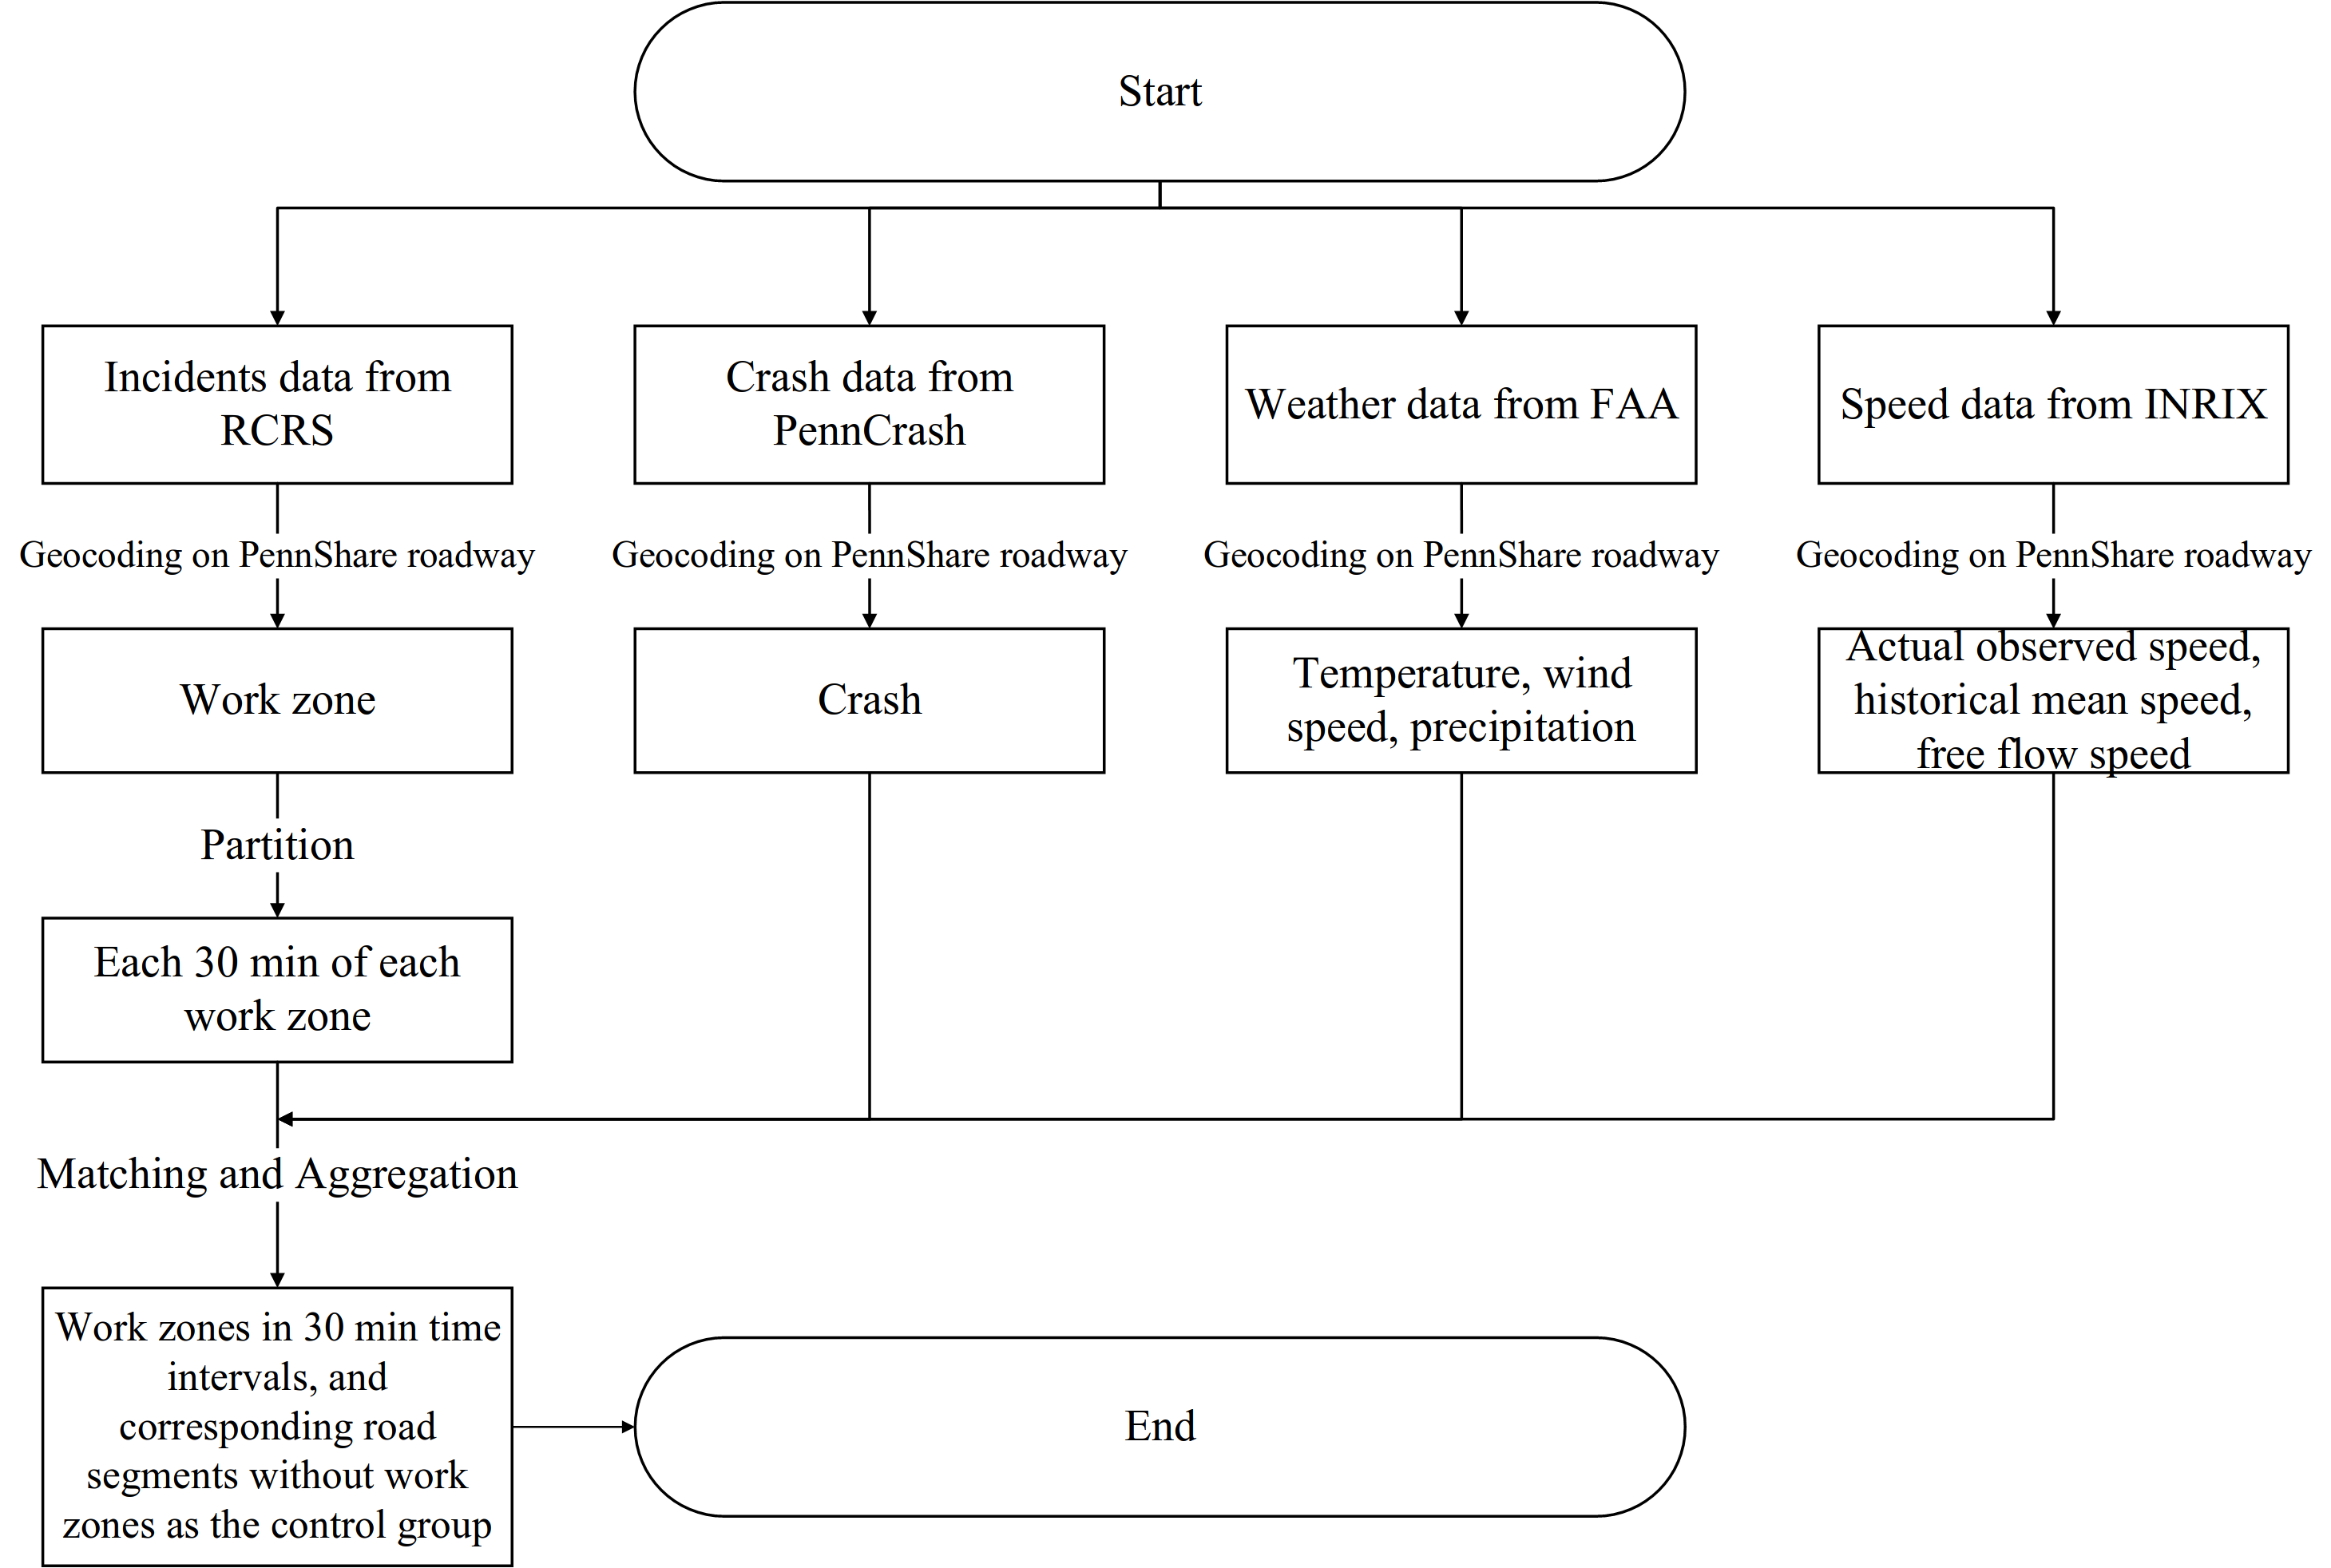
\includegraphics[width=1\textwidth]{media/rq1/DataProcessing3.png}
  \caption{Data processing workflow}\label{fig:rq1-1:dataprocessingflow}
\end{figure}

Figure~\ref{fig:rq1-1:dataprocessingflow} presents the workflow of data processing.
  
